\setcounter{section}{0}

\Needspace{5\baselineskip}
\hypertarget{multi-token-prediction}{%
\section{Multi-token Prediction}\label{multi-token-prediction}}

\Needspace{5\baselineskip}
\hypertarget{ux4e00multi-token-predictionmtpux7684ux63d0ux51faux80ccux666f}{%
\subsection{一、Multi-Token Prediction（MTP）的提出背景}\label{ux4e00multi-token-predictionmtpux7684ux63d0ux51faux80ccux666f}}

由于LLM的推理是自回归的，每次生成一个token，都要在显存中加载一轮完整的模型参数，导致显存带宽成为推理速度的显著瓶颈。同时，在利用Next token prediction进行训练的过程中，模型只能学习基于当前预测下一个token的质量，而无法拥有更远的``视野''。Multi-Token Prediction（MTP）通过在训练和推理中每一次并行生成多个token，来解决这些问题。

\Needspace{5\baselineskip}
\hypertarget{ux4e8cblockwise-parallel-decoding}{%
\subsection{二、Blockwise Parallel Decoding}\label{ux4e8cblockwise-parallel-decoding}}

这是Google于2018年提出的范式，也是MTP的初始形态。

\Needspace{4\baselineskip}
\begin{enumerate}
\def\labelenumi{\arabic{enumi}.}
\tightlist
\item
  模型架构
\end{enumerate}

\begin{figure}[htbp]
\centering
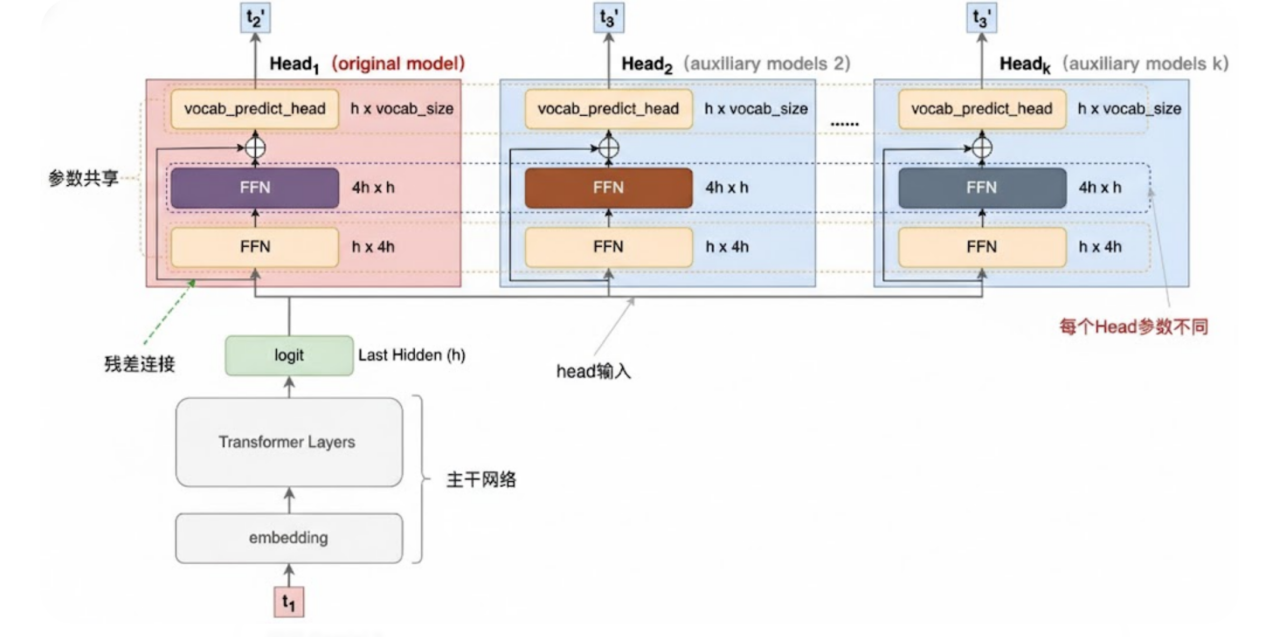
\includegraphics{images/image-0025.png}
\caption{Blockwise Parallel Decoding 模型架构图}
\end{figure}

如图，主干网络是训练好的多层decode-only的Transformer网络，经过多层前向计算后，最终隐藏层输出h维度（＝embedding维度）的logit。上面接了多个输出Head，每个Head负责预估一个token。每个Head有三层：首先是一个共享的FFN层，将logit做宽映射（h维-\textgreater4h维）；然后再过一个非共享的FFN层，将logit维度还原（4h维-\textgreater h维），经残差连接，得到h维embedding向量。最后，再将结果送入到词表投影层得到每个词的概率分布。

\Needspace{4\baselineskip}
\begin{enumerate}
\def\labelenumi{\arabic{enumi}.}
\setcounter{enumi}{1}
\tightlist
\item
  生成范式
\end{enumerate}

\begin{figure}[htbp]
\centering
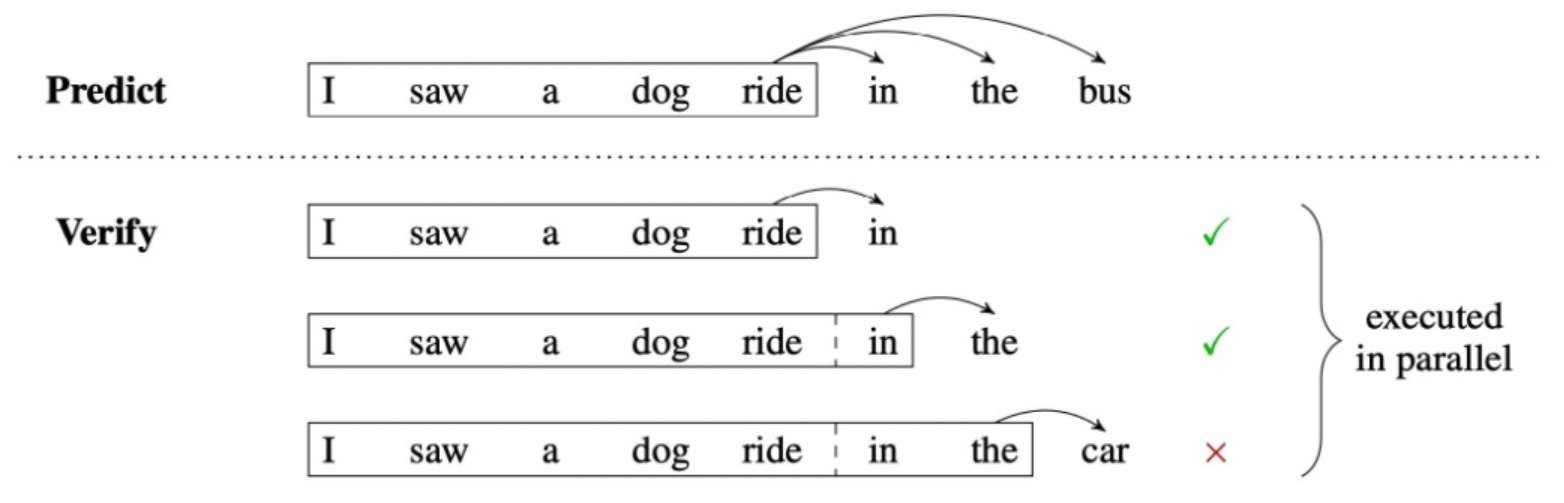
\includegraphics{images/image-0026.png}
\caption{Blockwise Parallel Decoding 的 Predict-Verify 生成与验证流程图}
\end{figure}

MTP的生成过程是一个``Predict-Verify''的循环过程。先一次性预测 \(K\) 个 token，然后利用Transformer的并行性，如图通过掩码的方式实现并行验证。如果预测全部正确，相当于用2次推理的时间实现了 \(K\) 次推理。

进一步地，重叠第 \(n\) 步的 verify 阶段和第 \(n+1\) 步的 predict 阶段，能进一步提高推理性能。如图，先预测出 3 个 token，然后在验证阶段，仍然每次都预测 3 个 token。如由于第 2 个正确，可以以其为条件生成第 3 个``car''、第 4 个``this''和第 5 个``week''，由于最初预测的第 3 个对不上，故最初的预测只能留下``in''和``the''，然后这里生成的第 3 到第 5 个 token 就可以直接作为新的一轮预测，后续再验证此时生成的第 4 和第 5 个，以此类推，不需要重新预测 3 个 token。

\begin{figure}[htbp]
\centering
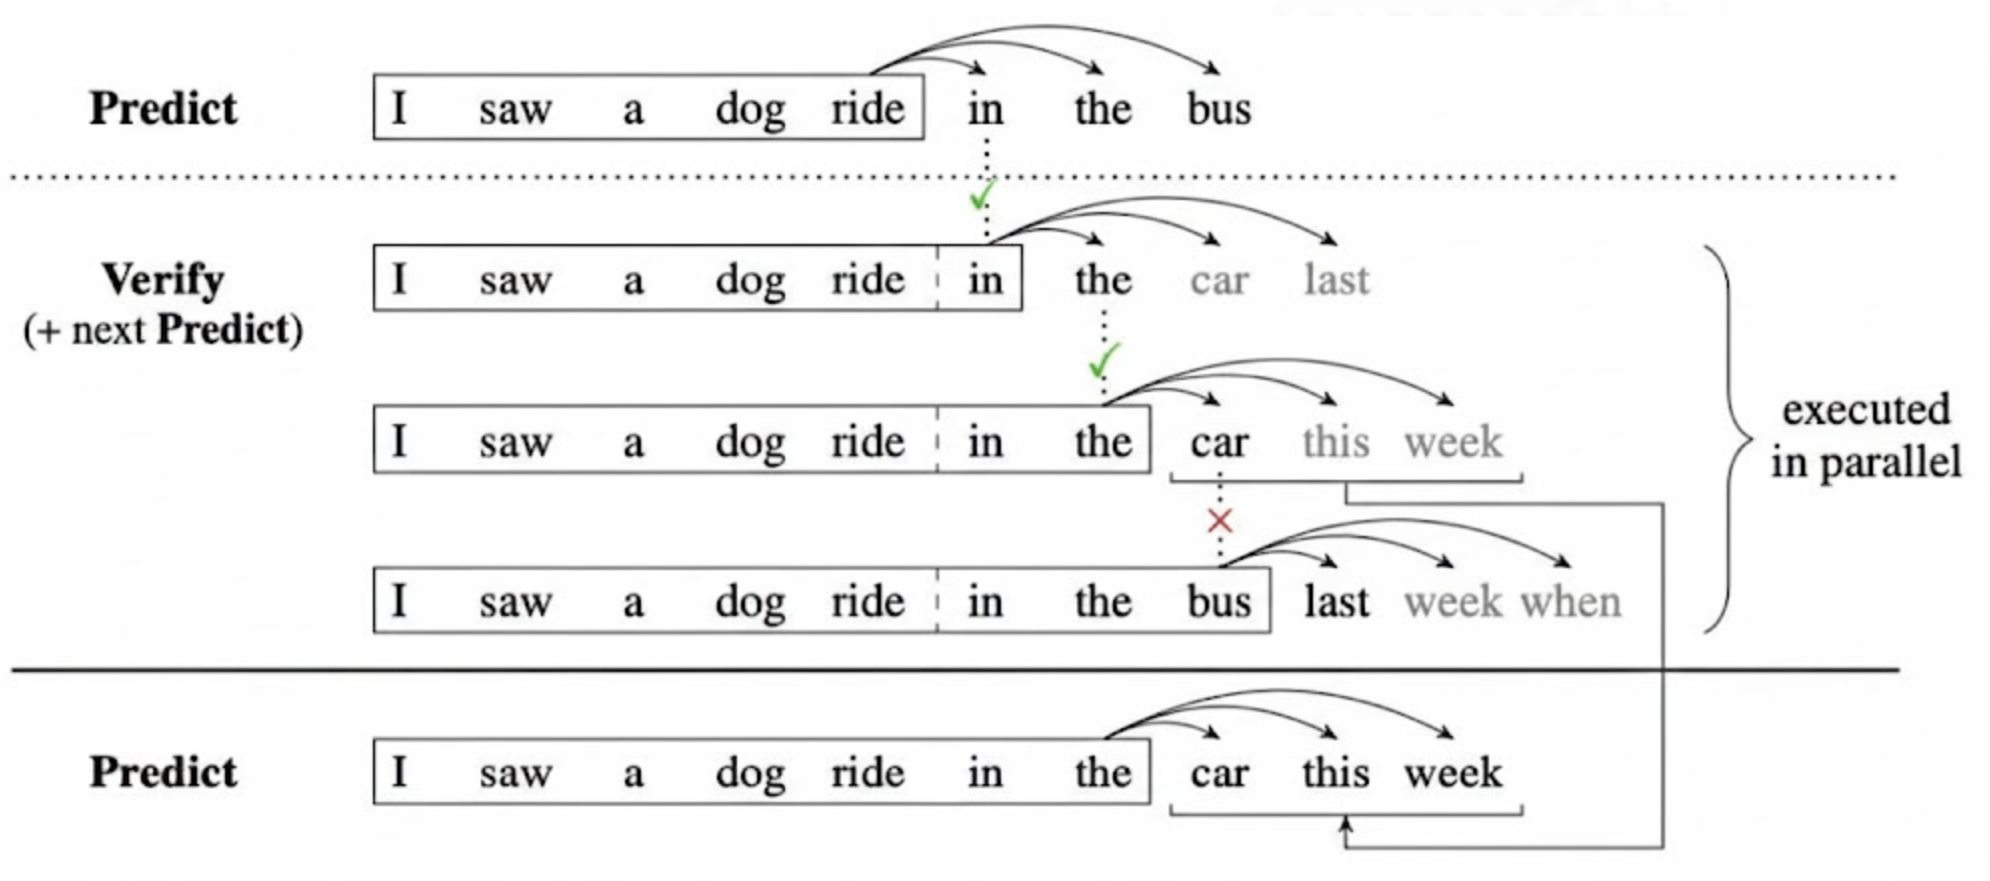
\includegraphics{images/image-0027.png}
\caption{Verify 与下一轮 Predict 重叠执行流程图}
\end{figure}

本质上，这就是利用多token生成的并行性，把后续根据``in''``the''这两个正确的token进行新一轮预测的步骤并入之前的验证步骤。

\Needspace{5\baselineskip}
\hypertarget{ux4e09metas-mtp}{%
\subsection{三、Meta's MTP}\label{ux4e09metas-mtp}}

如图，Meta让每个头不仅仅是FFN层，还有Transformer层，从而可以处理更复杂的序列上下文关系。

\begin{figure}[htbp]
\centering
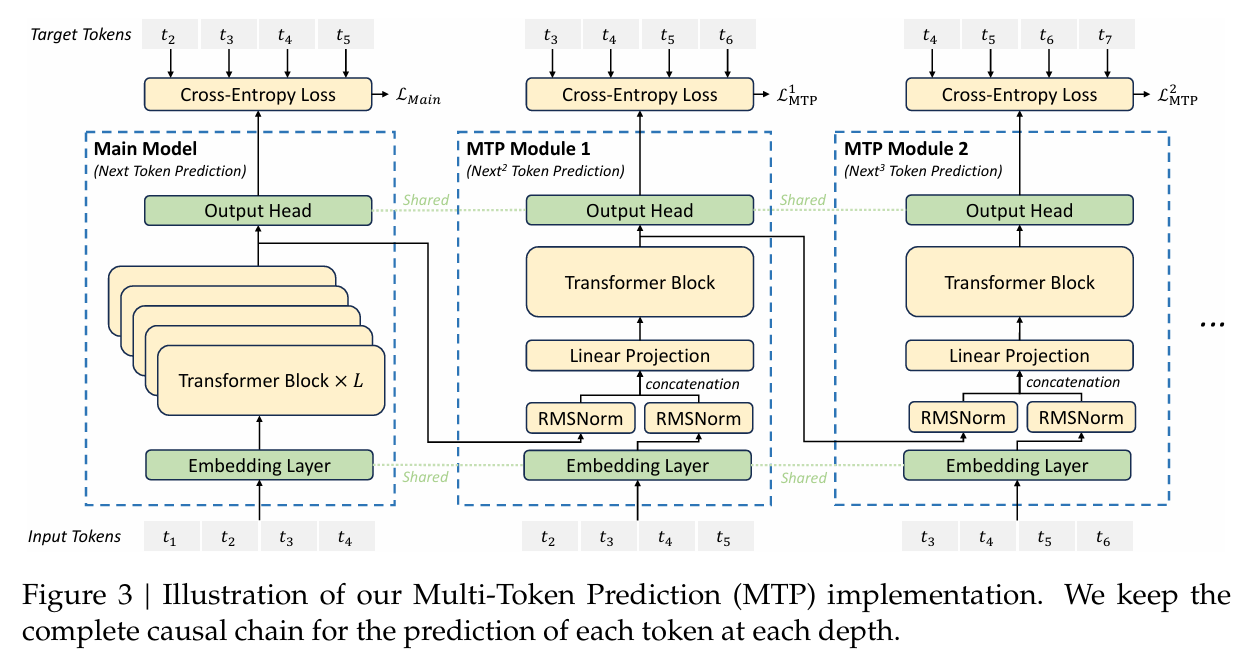
\includegraphics{images/image-0028.png}
\caption{Meta 的 Multi-token Prediction 架构图}
\end{figure}

\Needspace{5\baselineskip}
\hypertarget{ux56dbdeepseek-mtp}{%
\subsection{四、DeepSeek MTP}\label{ux56dbdeepseek-mtp}}

\begin{figure}[htbp]
\centering
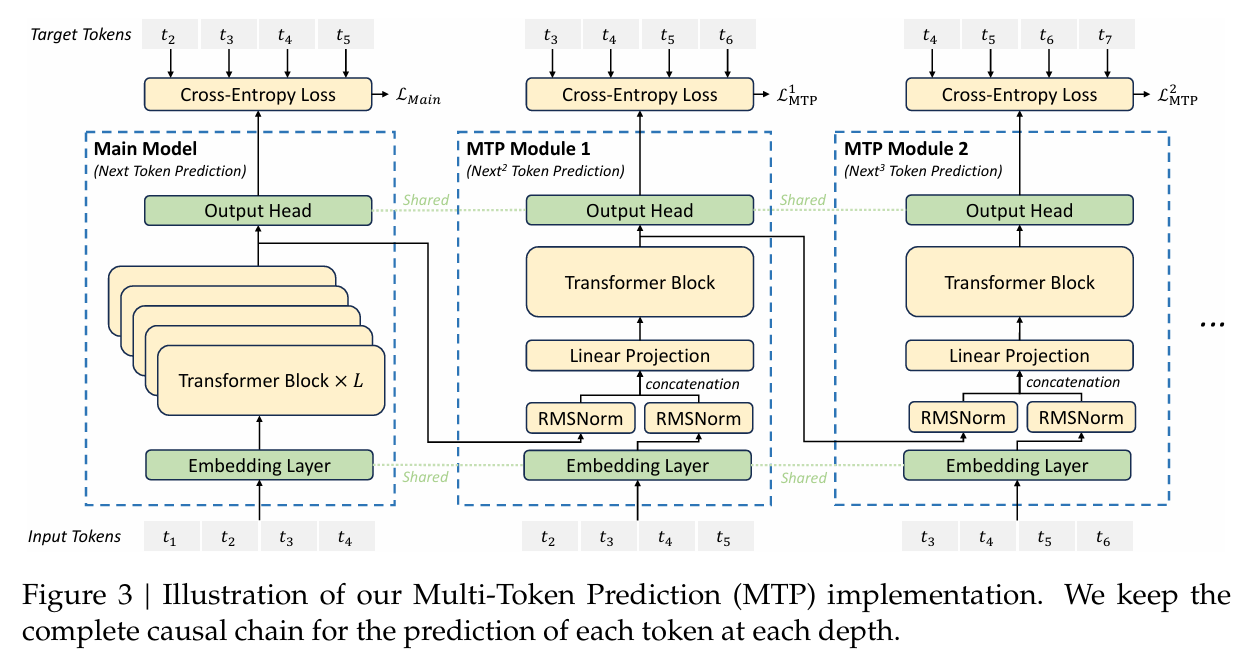
\includegraphics{images/image-0029.png}
\caption{DeepSeek MTP 训练样本构造图}
\end{figure}

训练阶段：Main Model：由 \(t_1\) 生成 \(t_2\)；由 \(t_1,t_2\) 生成 \(t_3\)；\ldots\ldots；由 \(t_1\) 到 \(t_{10}\) 生成 eos token；计算平均Cross-Entropy Loss。MTP Model 1：MTP Module：由 \(t_1,t_2\) 生成 \(t_3\)；\ldots\ldots；由 \(t_1\) 到 \(t_9\) 生成 eos token；计算平均Cross-Entropy Loss。后续的MTP Module以此类推。

\begin{figure}[htbp]
\centering
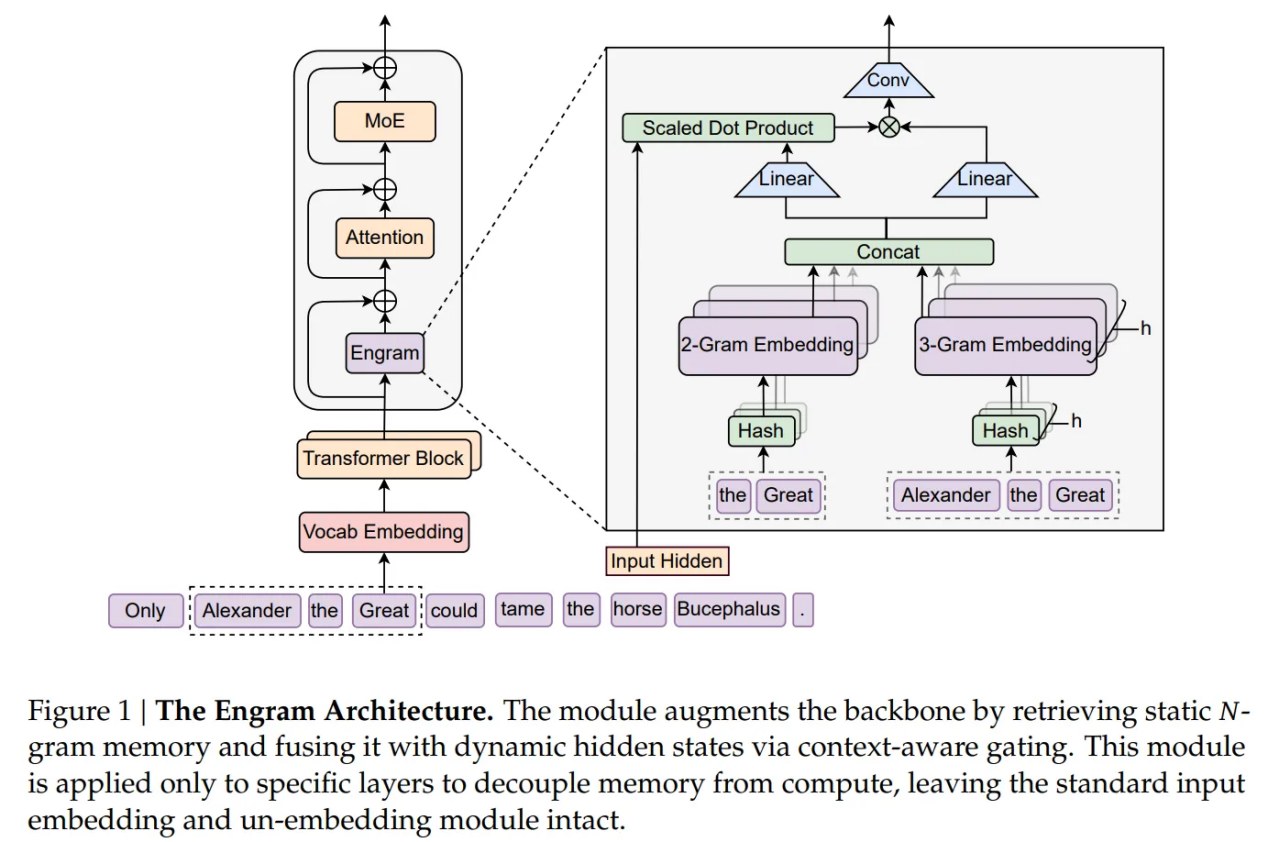
\includegraphics{images/image-0030.png}
\caption{DeepSeek MTP 模块架构图}
\end{figure}

\Needspace{5\baselineskip}
从模型架构上看，DeepSeek在Meta工作的基础上，还在MTP的Transformer层前加上了额外的输入。这个额外输入在训练时是ground truth的t2和t3，以防止细微误差导致``跑偏''；在推理时则是模型自身预测的t2和t3（虽然运用了上一次预测，但这里并非退化为Next token prediction，因为自身预测的t2和t3只经过轻量级MTP模块，不经过全模型，故仍为MTP）。MTP头的损失：

\[
\mathcal{L}_{\mathrm{MTP}}^k
= \mathrm{CrossEntropy}\left(P^k_{2+k:T+1}, t_{2+k:T+1}\right)
= -\frac{1}{T}\sum_{i=2+k}^{T+1}\log P_i^k[t_i].
\]

\Needspace{5\baselineskip}
DeepSeek原论文中插图如下：

\begin{figure}[htbp]
\centering
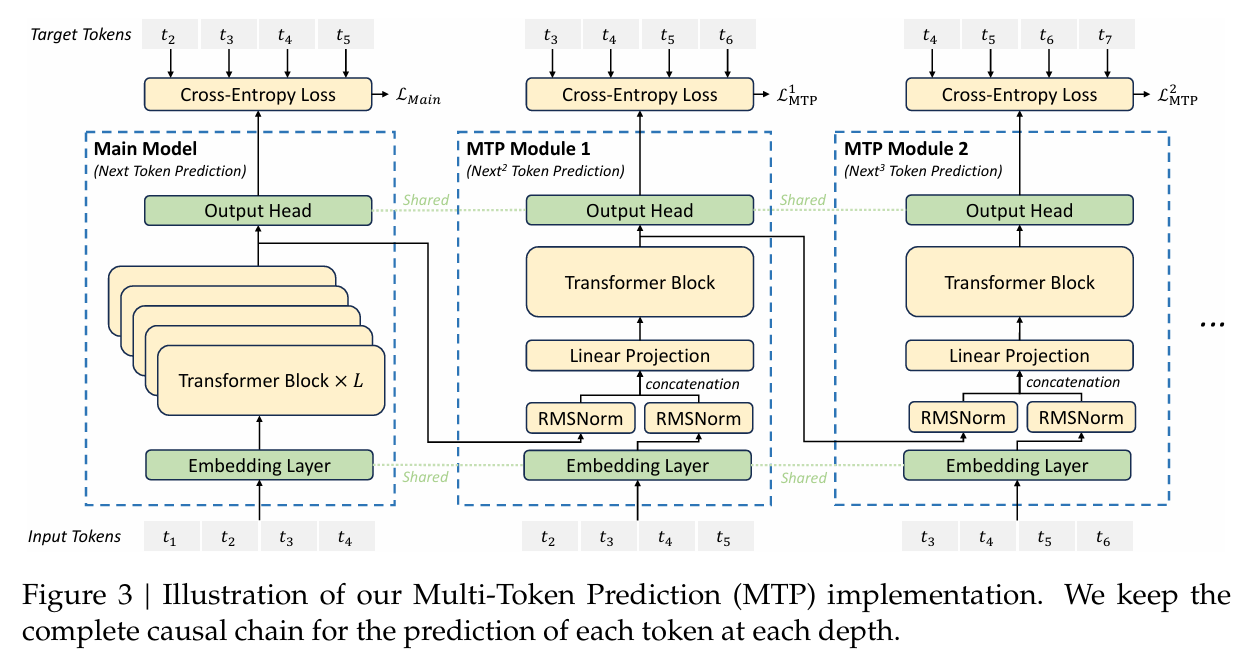
\includegraphics{images/image-0031.png}
\caption{DeepSeek 原论文中的 MTP 模块结构图}
\end{figure}

\FloatBarrier
\Needspace{5\baselineskip}
\hypertarget{ux53c2ux8003ux6587ux732e-101}{%
\subsection{参考文献}\label{ux53c2ux8003ux6587ux732e-101}}

\vspace{0.25em}
\begin{itemize}
\tightlist
\item
  Stern, M., Shazeer, N., \& Uszkoreit, J. (2018). \href{https://arxiv.org/abs/1811.03115}{Blockwise Parallel Decoding for Deep Autoregressive Models}. NeurIPS 2018.
\item
  Gloeckle, F., Idrissi, B. Y., Roziere, B., et al.~(2024). \href{https://arxiv.org/abs/2404.19737}{Better \& Faster Large Language Models via Multi-token Prediction}. ICML 2024.
\item
  DeepSeek-AI. (2024). \href{https://arxiv.org/abs/2412.19437}{DeepSeek-V3 Technical Report}. arXiv:2412.19437.
\item
  姜富春. (2025). \href{https://zhuanlan.zhihu.com/p/18056041194}{从DeepSeek V3的MTP，解析MTP技术的前世今生}. 知乎专栏.
\end{itemize}

\clearpage
